{\color{red} Deben definir los siguientes conceptos:}
\begin{itemize}
	\item \textbf{{\color{red}Conmutación}}
	\begin{itemize}
		\item \textbf{{\color{red}Circuitos}} \\
		La conmutación de circuitos se diseñó específicamente para la comunicación por voz y no es ideal para la transmisión de datos. En la conmutación de circuitos, se debe crear un canal dedicado entre el remitente y el receptor antes de que puedan hablar entre sí. \\{ }\\
		Se configura en la capa física, envía el mensaje completo a través del canal dedicado. Este tipo de conmutación no es ideal para la transmisión de datos porque los datos se envían y reciben en secuencias, lo que significa que la línea permanecería inactiva entre los períodos de transmisión. Eso sería una pérdida de ancho de banda.
		\\{ }\\
		\textbf{Fases de la conexión conmutada de circuito:}		
		\begin{itemize}
		\item \textbf{Establecimiento de circuitos:} en esta fase, se establece un circuito dedicado desde el origen hasta el destino a través de varios centros de conmutación intermedios. El remitente y el receptor transmiten señales de comunicación para solicitar y reconocer el establecimiento de circuitos. \\
		\item\textbf{ Transferencia de datos:} una vez que se ha establecido el circuito, los datos y la voz se transfieren desde la fuente al destino. La conexión dedicada permanece mientras las partes finales se comuniquen.\\
		\item \textbf{Desconexión del circuito:} cuando se completa la transferencia de datos, se abandona la conexión. La desconexión la inicia cualquiera de los usuarios. La desconexión implica la eliminación de todos los enlaces intermedios del remitente al receptor. \\
		\end{itemize}
		
\begin{figure}[ht!]
\centering
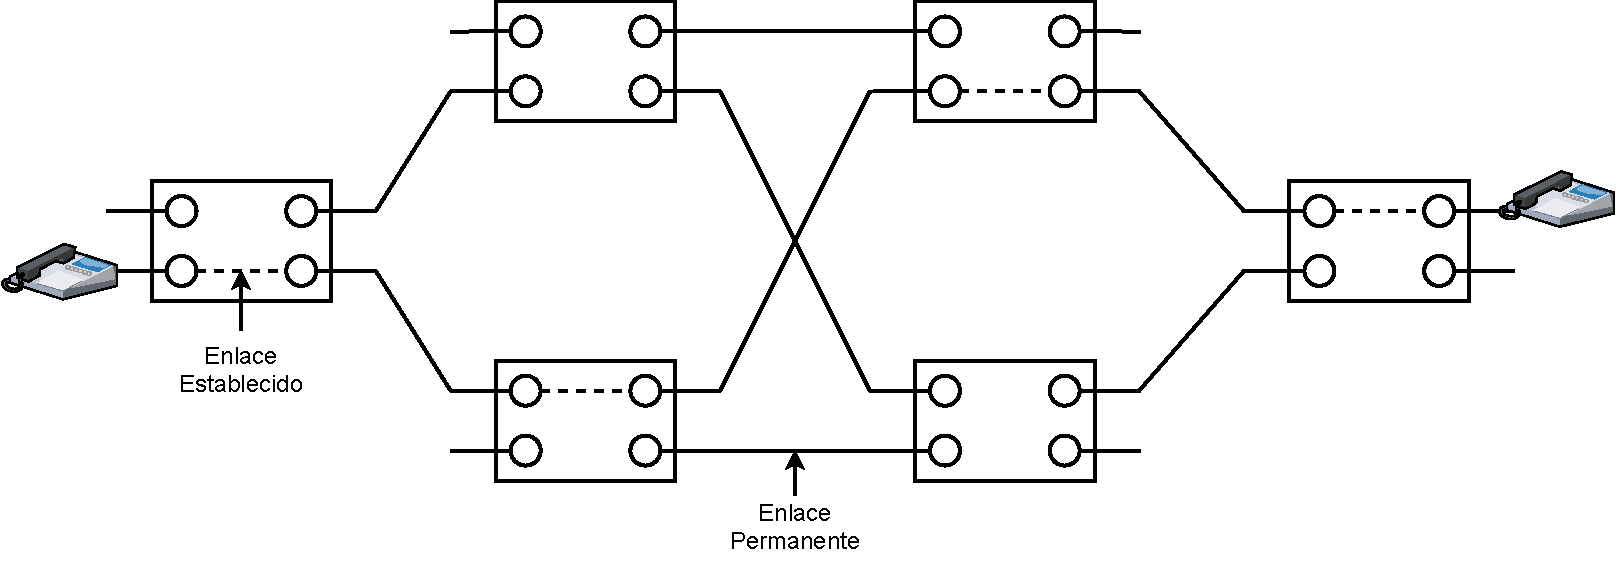
\includegraphics[scale=0.5]{Imagenes/circuito.pdf}
\end{figure}		
		
		\pagebreak
		\textbf{Ventajas y Desventajas}
		
		\begin{itemize}
		\item \textbf{Ventajas}
		\begin{itemize}
		\item Es adecuado para transmisiones continuas largas, ya que se establece una ruta de transmisión continua, que permanece durante toda la conversación.
		\item La ruta dedicada garantiza una velocidad de comunicación constante.
		\item No se encuentran retrasos intermedios una vez que se establece el circuito. Por lo tanto, son adecuados para la comunicación en tiempo real de transmisión de voz y datos.
		\end{itemize}
		\item \textbf{Desventajas}
		\begin{itemize}
		\item La conmutación de circuitos establece una conexión dedicada entre las partes finales. Esta conexión dedicada no se puede utilizar para transmitir ningún otro dato, incluso si la carga de datos es muy baja.
		\item El requisito de ancho de banda es alto incluso en casos de bajo volumen de datos.
		\item Hay subutilización de los recursos del sistema. Una vez que los recursos se asignan a una conexión en particular, no se pueden usar para otras conexiones.
		\item El tiempo necesario para establecer la conexión puede ser elevado.
		\end{itemize}
		\end{itemize}				
		
		\item \textbf{{\color{red}Paquetes}}\\
		La conmutación de paquetes es una técnica de conmutación de red sin conexión. Aquí, el mensaje se divide y se agrupa en varias unidades llamadas paquetes que se enrutan individualmente desde el origen al destino. No es necesario establecer un circuito dedicado para la comunicación. La conmutación de paquetes se utiliza con mayor frecuencia para aplicaciones de datos y voz que no son \textit{time-sensitive.} El rendimiento de Packet Switching se denomina \textit{Best Effort}. Si transmite de remitente a receptor, toda la red hará todo lo posible para llevar el paquete al otro extremo lo más rápido posible, pero no hay garantías de qué tan rápido llegará ese paquete. 

\begin{figure}[ht!]
\centering
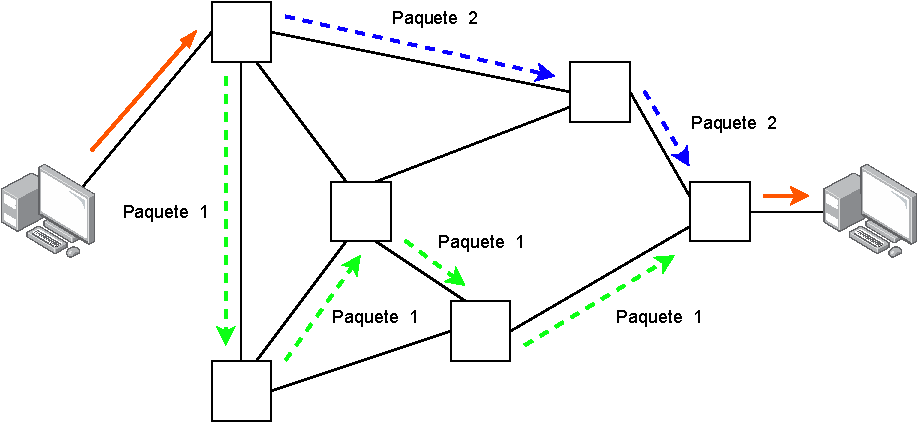
\includegraphics[scale=0.75]{Imagenes/paquete_ejemplo.pdf}
\end{figure}		
		
		\textbf{Formato de Paquetes}\\
		Un paquete contiene tres campos principales: \textit{el encabezado, el mensaje y los bits de verificación de redundancia.} Aparte de esos campos, puede tener otros campos que contribuyen a la conmutación.
				
\begin{figure}[ht!]
\centering
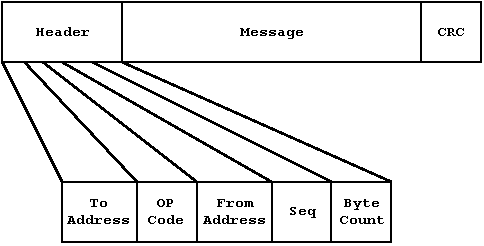
\includegraphics[scale=0.8]{Imagenes/paquete.pdf}
\end{figure}	
		\textbf{Ventajas y Desventajas}
	\begin{itemize}
		\item \textbf{Ventajas}
		\begin{itemize}
		\item Los paquetes de datos pueden encontrar el destino sin el uso de un canal dedicado.
		\item Reduce la pérdida de paquetes de datos porque la conmutación de paquetes permite el reenvío de paquetes.
		\item  Pueden transferir tráfico de red general y tráfico de voz a través de la red sin la necesidad de un canal dedicado. Esto permite ahorrar dinero porque no se necesita pagar para tener un canal disponible para las comunicaciones de voz.
		\end{itemize}
		\item \textbf{Desventajas}
		\begin{itemize}
		\item No es ideal para aplicaciones que están en uso constante, como llamadas de voz de alto volumen.
		\item Las redes de alto volumen pueden perder paquetes de datos durante tiempos de mucho tráfico; esos paquetes de datos no se pueden recuperar o reenviar durante la transmisión.
		\item Hay una falta de protocolos de seguridad para paquetes de datos durante la transmisión.
		\end{itemize}
	\end{itemize}			
		
		\item \textbf{{\color{red}Mensajes}}\\
		La conmutación de mensajes es una técnica de conmutación de redes sin conexión en la que todo el mensaje se enruta desde el nodo de origen al nodo de destino, un salto a la vez. Fue un precursor de la conmutación de paquetes.\\{ }\\ 
		\textbf{Proceso} \\
		La conmutación de paquetes trata cada mensaje como una unidad individual. Antes de enviar el mensaje, el nodo remitente agrega la dirección de destino al mensaje. A continuación, se entrega por completo al siguiente nodo de conmutación intermedio. El nodo intermedio almacena el mensaje en su totalidad, comprueba si hay errores de transmisión, inspecciona la dirección de destino y luego lo entrega al siguiente nodo. El proceso continúa hasta que el mensaje llega al destino. \\
		
		En el nodo de conmutación, el mensaje entrante no se descarta si el circuito saliente requerido está ocupado. En cambio, se almacena en una cola para esa ruta y se retransmite cuando la ruta requerida está disponible. Esto se denomina red de almacenamiento y reenvío.\\{ }\\
		\textbf{Ventajas y Desventajas}\\
		\begin{itemize}
			\item \textbf{Ventajas}
			\begin{itemize}
				\item    Reduce la congestión de la red debido al método de almacenamiento y reenvío. Cualquier nodo de conmutación puede almacenar los mensajes hasta que la red esté disponible.
				\item No tiene que lidiar con paquetes fuera de orden o paquetes perdidos como en la conmutación de paquetes.
			\end{itemize}
			\item \textbf{Desventajas}
			\begin{itemize}
				\item El método de almacenamiento y reenvío introduce un retraso en cada nodo de conmutación. Esto lo vuelve inadecuado para aplicaciones en tiempo real.
				\item Cada nodo de conmutación intermedio requiere una gran capacidad de almacenamiento.
			\end{itemize}
		\end{itemize}
		
		
	\end{itemize}

		
	
	\item \textbf{{\color{red}Handover}}\footnote{El término \textit{handover} es más común en publicaciones y literatura de investigación académica, mientras que \textit{handoff} es un poco más común dentro de las organizaciones IEEE y ANSI.} \\
	Se refiere al proceso de transferir una llamada en curso o una sesión de datos de un canal conectado a la red central a otro canal. \\{ }\\
	\textbf{Propósito}
	\begin{itemize}
	\item Cuando el teléfono se aleja del área cubierta por una celda y entra en el área cubierta por otra celda, la llamada se transfiere a la segunda celda para evitar la terminación de la llamada cuando el teléfono sale del alcance de la primera celda;
	\item Cuando la capacidad para conectar nuevas llamadas de una celda determinada se agota y una llamada nueva o existente de un teléfono, que se encuentra en un área superpuesta por otra celda, se transfiere a esa celda para liberar algo de capacidad en el primera celda para otros usuarios, que solo pueden conectarse a esa celda.
	\end{itemize}		
	
	\begin{itemize}
		\item \textbf{{\color{red}Hard}}\\
		Cuando hay una interrupción real en la conectividad al cambiar de una estación base a otra. No hay ninguna carga para la estación base y el MSC porque la conmutación se realiza con tanta rapidez que los usuarios apenas pueden notarlo. La calidad de la conexión no es tan buena. Hard Handoff adoptó la política de "romper antes de hacer". Libera el canal en la celda fuente y solo entonces se activa el canal en la celda objetivo. Por lo tanto, la conexión con la fuente se interrumpe antes o cuando se establece la conexión con el destino.
		
		\begin{figure}[ht!]
\centering
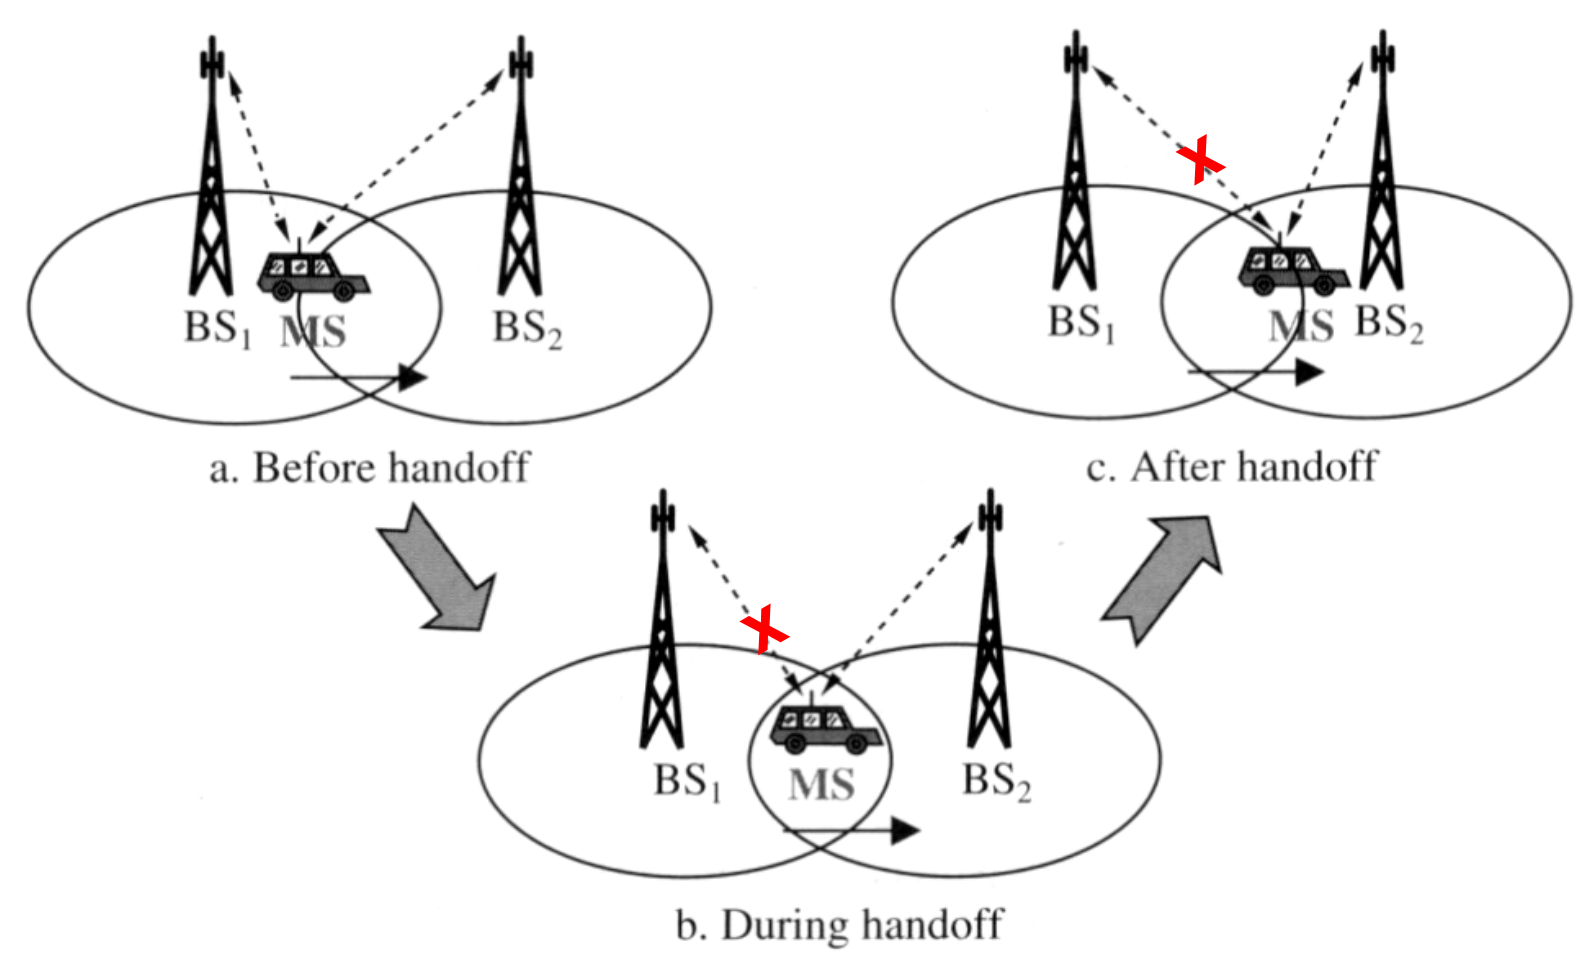
\includegraphics[scale=0.5]{Imagenes/hard.png}
\end{figure}	
		\item \textbf{{\color{red}Soft}}\\
		En Soft Handoff, al menos uno de los enlaces se mantiene cuando se agregan o eliminan señales de radio a la estación base. Soft Handoff adoptó la política de "hacer antes de romper". Soft Handoff es más costoso que Hard Handoff. El canal de la celda de origen se retiene y se usa durante un tiempo en paralelo con el canal de la celda de destino. En este caso, la conexión con el destino se establece antes de que se interrumpa la conexión con el origen.
				\begin{figure}[ht!]
\centering
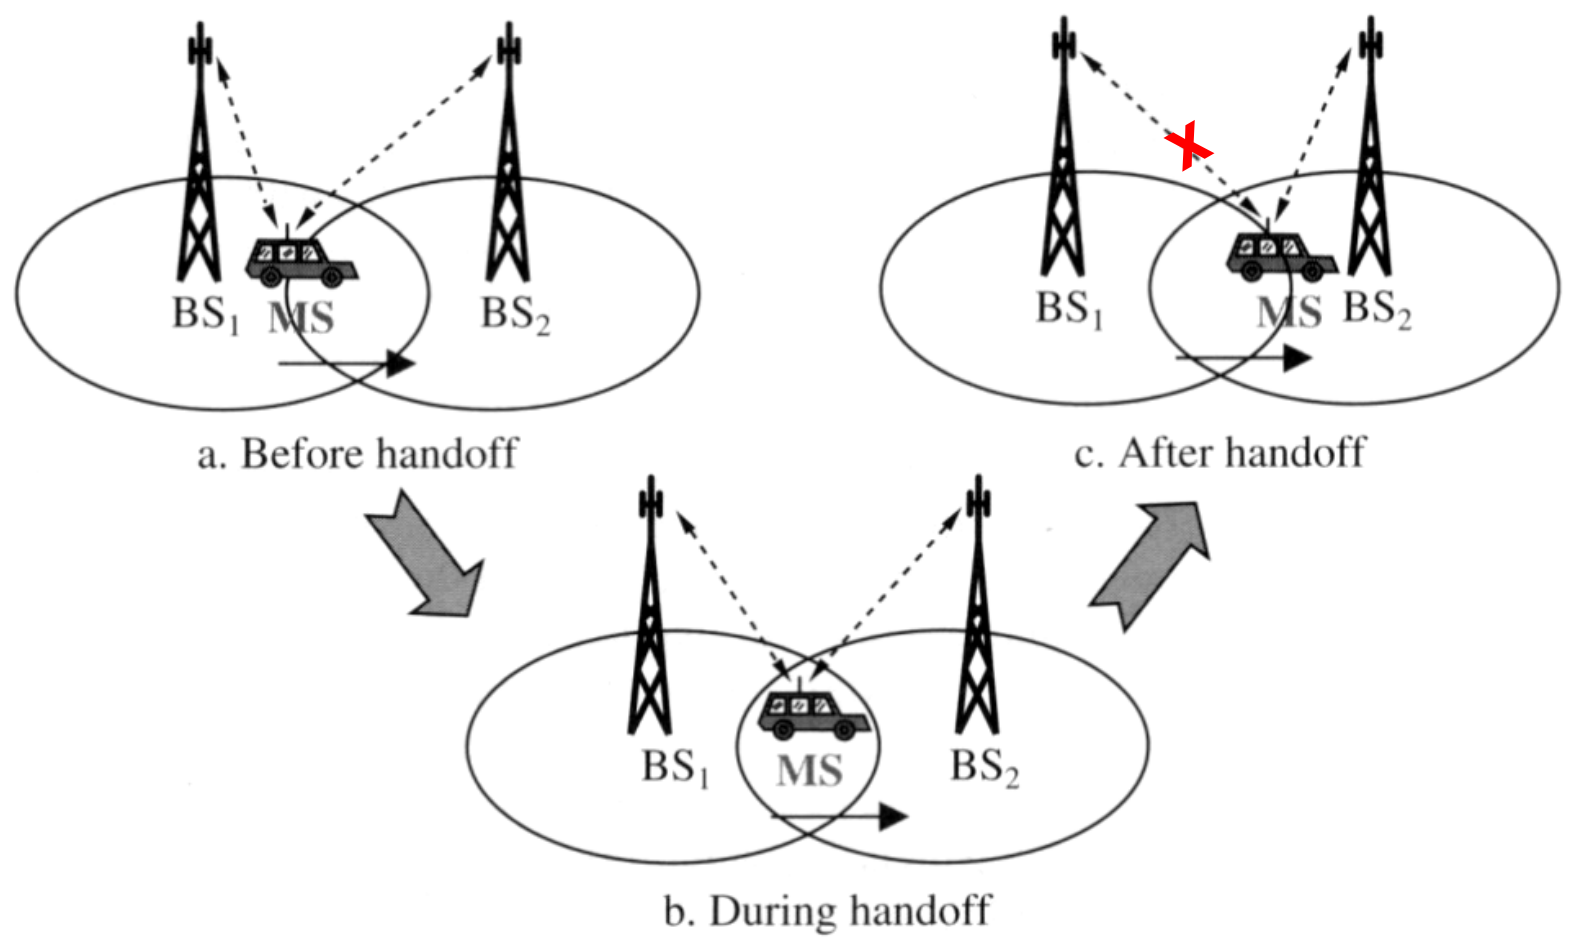
\includegraphics[scale=0.5]{Imagenes/soft.png}
\end{figure}	
	\end{itemize}
\end{itemize}


\begin{thebibliography}{9}
\bibitem{tutorialspoint} 
Circuit Switching \href{https://www.tutorialspoint.com/circuit-switching}{https://www.tutorialspoint.com/circuit-switching}

\bibitem{datto} 
What’s The Difference Between Circuit vs. Packet Switching. \href{https://www.datto.com/library/whats-the-difference-between-circuit-vs-packet-switching}{https://www.datto.com/library/whats-the-difference-between-circuit-vs-packet-switching} 31 de Marzo, 2020.


\bibitem{tutorialspoint2} 
Packet Switching. \href{https://www.tutorialspoint.com/packet-switching}{https://www.tutorialspoint.com/packet-switching}



\bibitem{dallas} 
Packet Switching and Computer Networks. Prof Morat Torlak\\ \href{https://ece.utdallas.edu/~torlak/courses/ee4367/lectures/packet.pdf}{https://ece.utdallas.edu/~torlak/courses/ee4367/lectures/packet.pdf}.


\bibitem{comparitech} 
Circuit Switching vs Packet Switching: Differences, Advantages \& Disadvantages. \href{https://www.comparitech.com/net-admin/circuit-switching-vs-packet-switching/}{https://www.comparitech.com/net-admin/circuit-switching-vs-packet-switching/}. 26 de Junio, 2020.


\bibitem{tutorialspoint3} 
Message Switching. \href{https://www.tutorialspoint.com/message-switching}{https://www.tutorialspoint.com/message-switching}.


\bibitem{handoff} 
Handoff in Cellular Telecommunications. \href{https://www.geeksforgeeks.org/handoff-in-cellular-telecommunications/}{https://www.geeksforgeeks.org/handoff-in-cellular-telecommunications/}.

\bibitem{NCKU} 
``Wireless \& Mobile Networks'', NCKU. Prof. W.-G. Teng. 

\end{thebibliography}

